\documentclass[10pt,twocolumn]{article}
\usepackage{amsthm, amssymb, geometry, mathrsfs}
\usepackage[T1]{fontenc}
\usepackage{graphicx}
\usepackage[utf8]{inputenc}
\usepackage[style=ieee]{biblatex}
\newcommand{\argmax}{\operatornamewithlimits{argmax}}
\addbibresource{citations.bib}
\usepackage{multicol}% http://ctan.org/pkg/multicols

\title {COMP 598: Multi-Class Classification of Reddit comments.}
\author {Xavier Denis, Ian Forbes, Liu Liu}

\begin {document}

\twocolumn[
\maketitle
\section{Abstract}
In this paper we collect a new machine learning dataset from the online social network Reddit. Consisting of 100 recent posts, with comments taken from each of the 9 most popular subreddits, this dataset provides new  questions. We implement a Naive Bayes classifier to classify the subreddit which the comment belongs. This classifier achieves 80\% performance in binary classification of 80,000 comments with 10-fold cross validation. When comparing 6 classes of 35k-94k comments each, it achieves 50\% performance. This work presents the possibility of recommending subreddits automatically based off of a user's comment history on Reddit.
\\
\\
]
\section{What is Reddit?}

Reddit is a popular online link aggregation website. It allows user to both post links to other webpages, images, videos, and more and to vote on the popularity of these submissions. Popular submissions are `Upvoted' while unpopular ones are `Downvoted'. Users are also allowed to comment on and discuss submissions. Comments, like submissions, can also be voted on. Some of the key vocabulary of Reddit is listed below.

\begin {enumerate}
\item \textbf{Post:} Also know as a submission is a link to another webpage. This webpage may be a news article, a blog post, an image, a video, etc. All posts contain a comment section where user are allowed to discuss the submission.
\item \textbf{Self Post:} Is a special type of post where a user writes their own text submission. This is often used to started discussions or ask questions in a given subreddit. 
\item \textbf{Subreddit:} A subsection of Reddit dedicated to a certain topic. 
\item \textbf{Upvote \& Downvote:} The action of voting on the popularity of a comment or post in either a positive or negative manner.
\item \textbf{Top level comment:} The root of a comment tree.
\end {enumerate}

\section{Motivation}
With the rise of social networks, many researchers have poured over the data produced to find and explore the connections between friends, text, and social interactions. While much research has been done on networks such as Twitter and Facebook, Reddit has remained largely ignored. The different structure of Reddit allows for an opportunity to look at different questions and a different style of conversation. Because Reddit users can label comments and posts as good or bad through voting, we can attempt to predict the interests of Reddit users.

Reddit also offers easy access to data for research and non-commercial purposes through it's API.\cite{reddit}. 

\begin{figure*}
    \centering
  	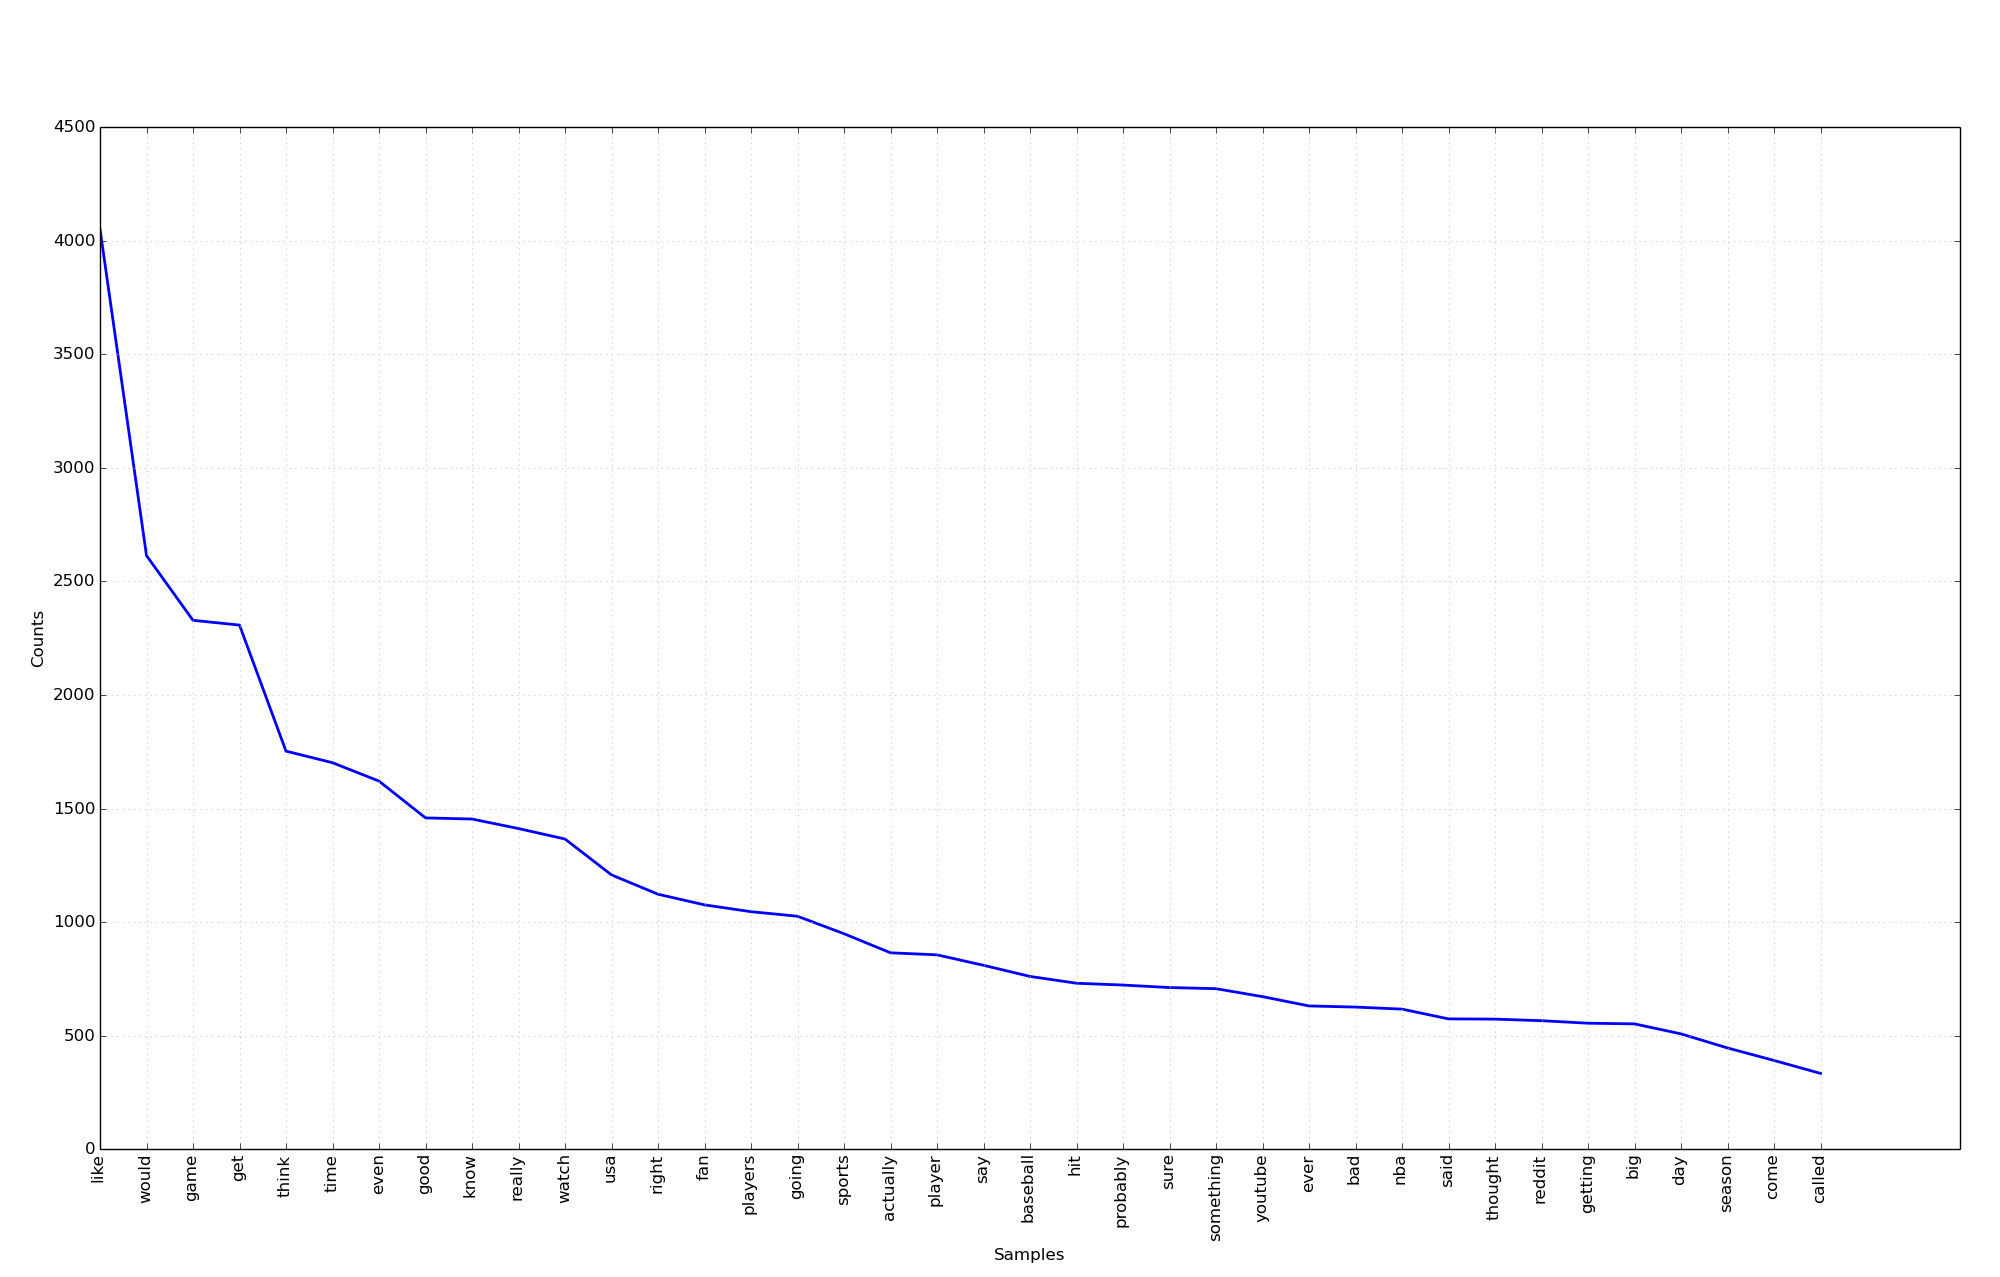
\includegraphics[width=0.92\textwidth]{./sports_freq.png}
  	\caption{Word frequency of the Sports subreddit.}
  	\label{sports}
\end{figure*}

\section{Related Work}

Due to the lack of studies related to Reddit there are few related datasets or papers. A search through Google Scholar produces few results and the top links are only listed because of share buttons on the paper's hosting site. Most of the related research we found were University projects like our own. We could not find any published papers or data.

However, we did find an interesting analysis\cite{bcjordan}as that aimed to predict the popularity of a self post based on its Flesch-Kincaid\cite{flesch1949art} readability. This project found a correlation between how easy a self post was to read and how popular it would be. In particular posts with moderate readability where more popular than others with easy or hard readability.

Our classification problem also has a stark resemblance to the 20 news groups problem of \cite{joachims1996probabilistic}. This paper is the original 20 news groups paper and compares the performance of various classification algorithms. The paper presents a Text Frequency - Inverse Document Frequency (TF-IDF) algorithm as well as a probabilistic variation on this algorithm. The authors compared the performance of these two algorithms, along with a naive Bayes classifier, to gauge their relative performance. In the end the performance of the algorithms was as follows.
\\

\begin{center}
\begin{tabular}{|c|c|}
\hline
Probabilistic TF-IDF & 90.3 \\
Naive Bayes & 88.6 \\
TD-IDF & 82.3 \\
\hline
\end{tabular}
\end{center}

\section{Dataset Description}

Reddit's developer API allowed us to download all of the post and comment data into structured JSON files. Each post is saved in a JSON file under its primary identifier. Each data file consists of 2 main parts, the meta data and the comments. The meta data contains information about the post, such as how many comments there are, the score of the post, a link to the content and the type of content (image, video, article, etc.). The comments section consists of a list the top level comments for that post. Each of the top level comments contains a list of of child comments (replies) which in turn may have their own children. 

In order to train our naive Bayes classifier we had to flatten the comments and evaluate the global word frequency for all the posts, creating a unigram frequency matrix for each post with comments as rows and features as columns.

\section{Methods}

We used a Naive Bayes classifier with single words (unigrams) as the features. We choose this classifier with the given feature set because the feature space, all words, is extremely large. Given that naive Bayes' complexity is linear with respect to the number of features we believe this to be a good choice \cite{hastie2009elements}. Our choice of feature set stems from the simplicity and speed of extracting single words from the text. This consisted of splitting the text on spaces and removing punctuation. 

Other possible features sets that we considered but were not adopted were bigrams and term frequency–inverse document frequency (TF-IDF)\cite{salton1983introduction}. One of the difficulties with bigrams is that they increase the sparseness of the features. This fact couple with the nature of most reddit comments, short - with poor spelling, grammar, and punctuation, weighed against the perceived usefulness of bi-grams when compared to uni-grams.

The other feature set we considered  was TF-IDF. This compares the ratio between the frequency of a word in a document and its total frequency in the text corpus. This gives another way to calculate the word frequency but penalizes words which are common among all documents in the corpus. Unfortunately, we only learned of this method towards the deadline and did not have time to implement it.

The naive Bayes classifier is a simple probabilistic classifier that relies on Bayes' rule and the assumption that features are conditional independent \cite{bishop2006pattern}. While this generaly untrue it has been shown to be quite accurate in practice. The output of the classifier is the probability that a given set of features $f_1,f_2,...f_n$ belong to the class $C$. When expressed together with Bayes' rule we get the following (Fig 2).

\[ Pr(C|f_1,f_2,...f_n) = \frac{Pr(C) \cdot Pr(f_1,f_2,...f_n|C)}{Pr(f_1,f_2,...,f_n)} \]

Now we can simplify the equation by invoking our independence assumption about the features. This leaves us with

\[ Pr(C|f_1,f_2,...f_n) =  Pr(C) \cdot \prod_{i=0}^{n} Pr(f_i|C) \]

Note that since $Pr(f_1,f_2,...,f_n)$ does not depend on $C$, and we are trying to maximize over $C$, we can consider it to be constant.

Thus the final goal of the classifier is:

\[ argmax_c (C) = Pr(C) \cdot \prod_{i=0}^{n} Pr(f_i|C) \]

For our classifier we used Laplace smoothing since some words are not observed in the training data for the classifier. The maximum likelihood estimator for the classifier was,
\[
Pr(x_i|y=C) = \frac {\Pr[x_i=1 \land y=1]+1}{\Pr[y=1]+2}
\]
Therefore, if there are no feature words from that class, the prior probability will be $0.5$, this prior avoids making any assumptions about the likelyhood of observing a word in the dataset \cite{bishop2006pattern}.

\subsection*{Multi-class classification}
We used a single classifier to compute $P(C|f_1,f_2,...f_n$) for each class, and selected the class with highest probability.
The other option is to use k different 1-vs-all binary classifiers. However, this method is computationally slower since many classifiers need to be learned, and the binary classes are imbalanced as the target class has relatively fewer data points compared to the aggregation of all the other classes.

\begin{figure}
    \centering  
    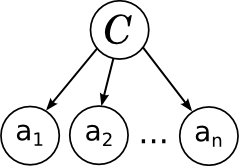
\includegraphics[width=0.5\textwidth]{./sysmag_bayes.png}
    \caption{Graphical representation of dependance in the Naive Bayes model. $C$ is the class and $a_i$ are the features. Readers should note that $C$ is dependent of the features but there is no dependence between features. }
    \label{bayesnet}
\end{figure}

\subsection*{Features selection and cross validation method}
For our features, we selected 2500 most frequently occurring single words, more specifically, unigrams, in the entire dataset to generate a features dictionary. Unigram were used as features, since bigrams can be sparse in the comments (Go et al. 2009). Also, reddit comments are likely to not follow standard grammar and/or spelling rules, therefore, unigram features with single words or part of words are optimal.
To validate our results we performed 10-fold cross validation on our classifier (Fig \ref{multiclass}). We divided the data, i.e. comments, from each subreddits, into 10 groups at random. The naive Bayes classifier was built from the data from 9 groups and the features from all the data. The classifier was then used to predict the subreddit(s) for the comments in the group left out and measure the prediction error. This training and testing procedure was repeated 10 time for each group to provide the final 10-fold cross-validation measure of the prediction error.

For classification problems with large number of features, that’s far greater than the number of data. This method might be prone to overfitting, since the full dataset was used to select the features. Therefore, we might have a slightly biased estimate of the generalization error in the testing set.

This can be avoided by selecting features only from the training data or from random samples of the data as discussed in class. These other options are computationally costly especially for large text dataset like ours, and might not be feasibly given limited time. Since we have a large data set with entirely 40,000-100,000 comments per subreddit and relatively small number of features, 2500, our cross-validation method might not be as prone to overfitting.

\section{Results}
\begin{figure}
    \centering
  	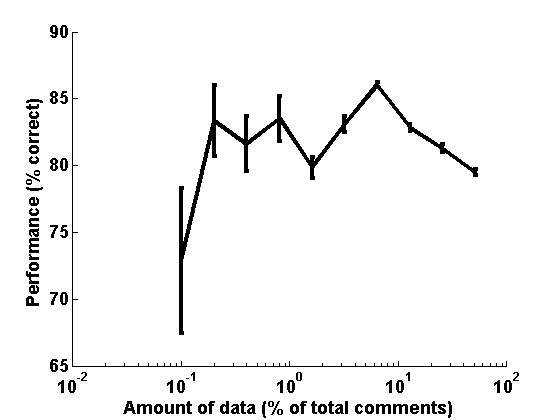
\includegraphics[width=0.5\textwidth]{./binary_data.png}
  \caption{ Binary classification performance as a function of the amount of data. There were a total of 35000 and 45000 comments in the two subreddits sports and books respectively. The performance was measure by 10-fold cross validation on the test data. The error bars represent the standard error of the 10 samples collected in the cross validation.}
  	\label{multiclass}
    \end{figure}
We obtained good classification performance with the naive Bayes classifier, attaining approximately $80\%$ (Fig \ref{multiclass}) in binary classification. The performance from cross-validation of the testing data is dependent on the amount of data. As the amount of data increased, the mean performance increased, and the variance decreased(Fig \ref{multiclass}). As the amount of classes increased, the performance dropped but stayed well above that of a random classifier (Fig \ref{classes}). Most importantly, by using a single classifier we avoided biasing the results towards any one class, resulting in a fairly uniform confusion matrix (Fig \ref{confusion}). While the amount of data in each class varied a lot but from the confusion matrix it is clear that there is no class that has been significantly over-fitted.


\begin{figure}
    \centering
  	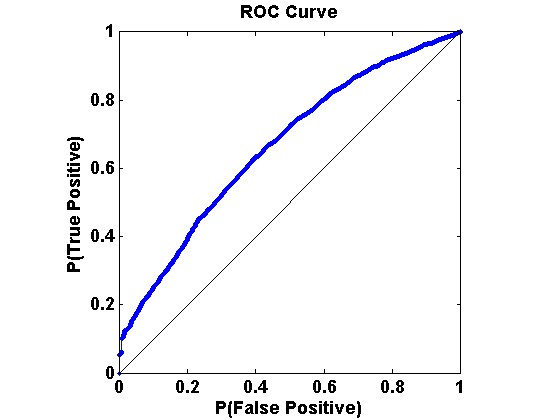
\includegraphics[width=0.5\textwidth]{./roc.png}
  	\caption{Receiver-operator characteristics (ROC) curve for binary classification performance using all the data. The classification threshold, i.e. decision boundary, of the naive Bayes classifier was defined by the log posterior of the test data.}
  	\label{roc}
\end{figure}		

\begin{figure}
    \centering
  	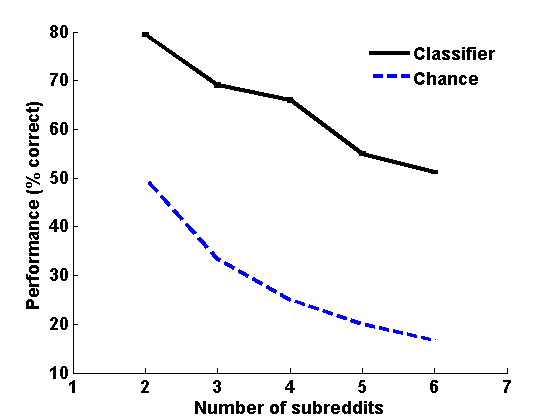
\includegraphics[width=0.5\textwidth]{./varyWBaseline.png}
  	\caption{Classifier performance as a function of the classes. The identity of the subreddit classes are in (Fig \ref{confusion})}
  	\label{classes}
\end{figure}	

\begin{figure}
    \centering
  	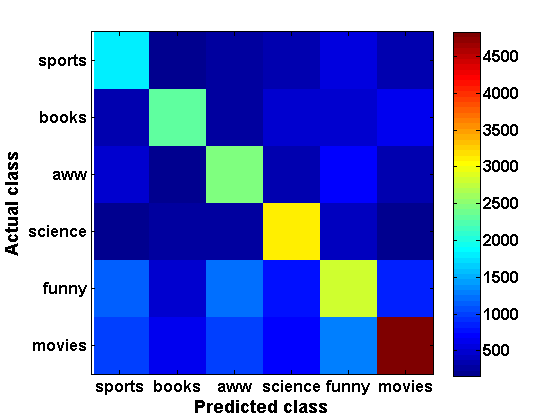
\includegraphics[width=0.5\textwidth]{./confusion_mat.png}
  	\caption{Confusion matrix for the multi-class performance. The number of comments in each subreddits is 35000, 45000, 46000, 46000, 73000, and 94000, respectively.}
  	\label{confusion}
\end{figure}	

\section{Discussion}
The final dataset and features are accurate when classifying but could still be improved. There were several issues during tokenization where standard approaches would fail due to Reddit's internal culture. The frequent use of non-textual unicode characters to encode emojis and other information wouldn't be captured by pure word tokenization. Additionally, the presence of Markdown\cite{gruber} for text formatting adds another level of complexity to the word extraction. We settled on stripping markdown formatting through Regular Expressions before splitting on spaces and stemming\cite{porter1980algorithm} words. However, there a few issues with things such as `l33tspeak' where numbers are subsistuted for letters, causing the stemmer to not recognize identical words. 

Overall our results were quite positive. A possible use of our classifier would be to recommend new subreddits to users based on their comment history. Each user's comments are publicly available on their profile so it would be very easy to classify each of the comments into a given subreddit. If a user's comments where consistently classified into a small subset of subreddits it is possble that they may be interested in that subreddit. On a larger scale, sometimes posts are added to the wrong subreddit, this classifier could detect that comments really belong in a different subreddit and automatically move the entire post to that subreddit where it could receive the appropriate community interaction.

We hereby state that all the work presented in the report is that of the authors.

\printbibliography
\section{Appendix}
\begin {enumerate}
\item \url{https://github.com/xldenis/proj1} - The complete project repository including data dictionary
\end{enumerate}
\end{document}